\documentclass[conference]{IEEEtran}

% Fix to revert the changes IEEEtran makes to table caption styles
\usepackage{etoolbox}
\makeatletter
\patchcmd{\@makecaption}
  {\scshape}
  {}
  {}
  {}
\makeatother
\usepackage[font=scriptsize,justification=justified,singlelinecheck=false]{caption}

%===========================================================================
\usepackage{listings}
\lstloadlanguages{C++,Pascal}

% Settings for the lstlistings environment
\lstset{
language=C++,                       % choose the language of the code
basicstyle=\footnotesize\ttfamily,  % the size of the fonts that are used for the
                                    % code
numbers=none,                       % where to put the line-numbers
numberstyle=\tiny,                  % the size of the fonts that are used for the
                                    % line-numbers
stepnumber=1,                       % the step between two line-numbers. If it's
                                    % 1 each line will be numbered
numbersep=5pt,                      % how far the line-numbers are from the code
%backgroundcolor=\color{gray},      % choose the background color. You must add
                                    % \usepackage{color}
showspaces=false,                   % show spaces adding particular underscores
showstringspaces=false,             % underline spaces within strings
showtabs=false,                     % show tabs within strings adding particular
                                    % underscores
keywordstyle=\bfseries\color{blue},  % color of the keywords
commentstyle=\color{darkgreen},     % color of the comments
stringstyle=\color{darkred},        % color of strings
captionpos=b,                       % sets the caption-position to top
tabsize=2,                          % sets default tabsize to 2 spaces
frame=tb,                           % adds a frame around the code
breaklines=true,                    % sets automatic line breaking
breakatwhitespace=false,            % sets if automatic breaks should only happen
                                    % at whitespace
escapechar=\%,                      % toggles between regular LaTeX and listing
belowskip=0.3cm,                    % vspace after listing
morecomment=[s][\bfseries\color{blue}]{struct}{\ },
morecomment=[s][\bfseries\color{blue}]{class}{\ },
morecomment=[s][\bfseries\color{blue}]{public:}{\ },
morecomment=[s][\bfseries\color{blue}]{public}{\ },
morecomment=[s][\bfseries\color{blue}]{protected:}{\ },
morecomment=[s][\bfseries\color{blue}]{private:}{\ },
morecomment=[s][\bfseries\color{black}]{operator+}{\ },
xleftmargin=0.1cm,
%xrightmargin=0.1cm,
}

\usepackage{color}
\usepackage{comment}
\usepackage{graphicx}
\usepackage{amsmath}
\usepackage{amsfonts}
\usepackage{hyperref}
\usepackage{cite}
\newcommand{\fix}[1]{{\bf \textcolor {red}{#1}}}
%===========================================================================
\begin{document}
\title{Solving Large Quantities of Small Matrix Problems on Cache-Coherent SIMD Architectures}

%===========================================================================
% author names and affiliations
% use a multiple column layout for up to three different
% affiliations
\author{
\IEEEauthorblockN{Bryce Lelbach, Hans Johansen, and Samuel Williams}
\IEEEauthorblockA{Computational Research Division, Lawrence Berkeley National Laboratory, Berkeley, CA 94720\\ {\it \{balelbach, hjohansen, swwilliams\}@lbl.gov}}
%\and
%\IEEEauthorblockN{Homer Simpson}
%\IEEEauthorblockA{Twentieth Century Fox\\
%Springfield, USA\\
%Email: homer@thesimpsons.com}
}

% conference papers do not typically use \thanks and this command
% is locked out in conference mode. If really needed, such as for
% the acknowledgment of grants, issue a \IEEEoverridecommandlockouts
% after \documentclass

% for over three affiliations, or if they all won't fit within the width
% of the page, use this alternative format:
% 
%\author{\IEEEauthorblockN{Michael Shell\IEEEauthorrefmark{1},
%Homer Simpson\IEEEauthorrefmark{2},
%James Kirk\IEEEauthorrefmark{3}, 
%Montgomery Scott\IEEEauthorrefmark{3} and
%Eldon Tyrell\IEEEauthorrefmark{4}}
%\IEEEauthorblockA{\IEEEauthorrefmark{1}School of Electrical and Computer Engineering\\
%Georgia Institute of Technology,
%Atlanta, Georgia 30332--0250\\ Email: see http://www.michaelshell.org/contact.html}
%\IEEEauthorblockA{\IEEEauthorrefmark{2}Twentieth Century Fox, Springfield, USA\\
%Email: homer@thesimpsons.com}
%\IEEEauthorblockA{\IEEEauthorrefmark{3}Starfleet Academy, San Francisco, California 96678-2391\\
%Telephone: (800) 555--1212, Fax: (888) 555--1212}
%\IEEEauthorblockA{\IEEEauthorrefmark{4}Tyrell Inc., 123 Replicant Street, Los Angeles, California 90210--4321}}




% use for special paper notices
%\IEEEspecialpapernotice{(Invited Paper)}




% make the title area
\maketitle

%===========================================================================
\begin{abstract}
A number of computational science algorithms lead to discretizations
  that require a large number of independent, small matrix solves.
Examples include small non-linear coupled chemistry and flow systems,
  one-dimensional sub-systems in climate and diffusion simulations, 
  alternating direction implicit pre-conditioners, and 
  semi-implicit time integrators, among others.
We present a performant approach for solving large quantities of 
  independent matrix problems on cache-coherent SIMD architectures. 
Unlike many vectorized or ``batched'' approaches that rely on reusing
  the matrix factorization across multiple solves, our algorithm supports
  the case of sets of matrices that are different, due to
  spatial variation or non-linear solvers, for example.
We demonstrate the approach with a prototypical tridiagonal matrix solver,
  derived from a 1D solver that is part of an implicit-explicit 
  finite difference discretization for a 3D advection-diffusion problem.
Performance is evaluated on several Intel architectures with different cache,
  vectorization, and threading features, and compared to theoretical
  roofline models across parameter studies.
We conclude that the approach is effective at optimizing both vectorization 
  and memory bandwidth, and improves on existing approaches for efficiently
  solving large numbers of small matrix problems.
\end{abstract}

% no keywords


% For peer review papers, you can put extra information on the cover
% page as needed:
% \ifCLASSOPTIONpeerreview
% \begin{center} \bfseries EDICS Category: 3-BBND \end{center}
% \fi
%
% For peerreview papers, this IEEEtran command inserts a page break and
% creates the second title. It will be ignored for other modes.
\IEEEpeerreviewmaketitle

%===========================================================================
\section{Introduction}
% 
One important class of problems in computational science is the solving
  of smaller-dimensional matrix subproblems that are duplicated across
  many degrees of freedom in a larger two or more dimension computation.
Several examples of this include: 
\begin{itemize}
\item Pointwise chemistry systems in the context of a larger, 
  flow simulations. 
Examples include geochemistry~\cite{??}, cloud microphysics~\cite{??},
  and combustion~\cite{??};
\item Solving one-dimensional systems that represent a ``primary''
  direction for a physical phenomenon.
Examples here include atmospheric radiation~\cite{??}, groundwater
  penetration~\cite{??}, or models for cloud convection~\cite{??}; and
\item Implicit solvers that need to couple these kinds of subsystems, 
  such as physics-based preconditioners~\cite{??}, alternating 
  direction implicit ADI,~\cite{??}, and operator-split or
  semi-implicit time integrators~\cite{??}.
\end{itemize}
In most cases, these matrices are relatively small 
  (ranging from $O(10-100)$ chemistry components or ``levels'' 
  in a climate application), and may be sparse or dense, but must 
  be solved repeatedly, but with different entries each time, 
  to advance the overall simulation.
Thus, because these are often non-linear matrix systems with space- and 
  time-dependent entries, these applications may not use a 
  ``factor once, solve many times'' approach, which is often used 
  as a model matrix performance test.
This prevents amortizing setup and factorization costs
  across multiple right-hand side solves as in \emph{dgxxxxx}~\cite{??},
  and also challenges SIMD vectorization due to the odd size and
  dissimilar entries of the matrices, as well as the 
  memory access patterns relative to the bigger simulation data layout.
In that case, it is usually sub-optimal on many-core SIMD 
  or SIMT GPU architectures
  to simply call an optimized linear algebra library, 
  such as Intel's MKL version of LAPACK~\cite{mkl_website} or NVIDIA's
  cuBLAS~\cite{cublas_website}; these may not achieve peak memory bandwidth 
  and VPU performance across the range of small matrix size. 
In that sense, it can leads applications to create their own 
  custom implementations, which may not be optimal, and create a 
  (potentially unnecessary) maintenance burden for the applications 
  running across multiple many-core architectures as well. 
  
To this end, we have developed a model matrix kernel that mimics what
  is encountered in these kinds of large-scale simulations.
Key aspects of the code include:
\begin{itemize}
\item Matrix systems that must be created and solved
  at each point in a two-dimensional subdomain (represented by $(i,j)$ indices)
  of a three-dimensional application (that is, $(i,j,k)$ indices).
\item Each matrix is tri-diagonal, and must be solved for all $O(30-100)$
  values in the $k$ index.
\item The matrix is derived from finite difference discretization for the
  1D diffusion equation, which allows it to be solved without pivoting
  (pivoting will be addressed in future work).
\end{itemize}

%===========================================================================
\section{Related Work}
Approaches to solving large numbers of small matrices have been done
  in a variety of contexts.
Many implementations simply solve each matrix in parallel or for multiple
  right-hand sides, using platform-specific
  implementations of LAPACK, such as Intel's Math Kernel Library~\cite{mkl_website}
  or NVIDIA's cuBLAS~\cite{cublas_website} implementations.
In many cases, there is a benefit from vectorization and thread parallelism, 
  but there may be overheads that reduce performance such as data copies
  into local arrays, dynamic determination of optimal performance parameters, 
  partially vectorized ``peel'' loops, etc.~\cite{??}.
Some specialized approaches include specialized linear algebra-specific 
  compilers for small problem sizes and target architectures 
 ~\cite{Spampinato:2014, ??} \fix{(add build-to-order ref, Siek/Jessup?)}.
Other libraries like 
  \emph{Blaze}~\cite{BlazeSite}, 
  \emph{PLASMA}~\cite{PLASMASite},
  \emph{MAGMA}~\cite{Haidar:2015}, and 
  \emph{libxsmm}~\cite{libxsmm_website}
  are intended to support SIMD vectorization for standard vector sizes
  as well as batched computation for sparse and dense matrices.
Overall, there is a gap in approaches that both have vectorization,
  regardless of matrix size, with or without dense/sparse/pivoting 
  assumptions, amortizing factorization across multiple right-hand-sides, 
  and other assumptions.
\\
\fix{(Hans - fill in more background / details on these.)}

%===========================================================================
\section{Implementation}
\fix{Bryce to write}

Suppose we have a symmetric positive-definite or diagonally-dominant $n$x$n$
tridiagonal matrix $A$ and two $n$-element vectors $u^{s}$ and $u^{s+1}$. We
wish to solve $Au^{s+1} = u^{s}$ for $u^{s}$:

\[
\begin{bmatrix}
b_0 & c_0 &     &         & 0       \\
a_1 & b_1 & c_1 &         &         \\
    & a_2 & b_2 & ...     &         \\
    &     & ... & ...     & c_{n-2} \\
0   &     &     & a_{n-1} & b_{n-1}
\end{bmatrix}
\begin{bmatrix}
u^{s+1}_0     \\
u^{s+1}_1     \\
...     \\
...     \\
u^{s+1}_{n-1}
\end{bmatrix}
=
\begin{bmatrix}
u^{s}_0     \\
u^{s}_1     \\
...     \\
...     \\
u^{s}_{n-1}
\end{bmatrix}
\]

Our matrix $A$ is stored as a set of three vectors: an $n-1$-element
sub-diagonal vector $a$, an $n$-element diagonal vector $b$ and an $n-1$-element
super-diagonal vector $c$.

We can use a simplified form of Gaussian elimination which does not perform any
pivoting to solve such a system. This method is known as the Thomas algorithm
or the tridiagonal matrix algorithm (TDMA)~\cite{TDMA}, and it is \(O(n)\) in time,
a significant improvement over full Gaussian elimination for a completely dense
matrix, which is \(O(n^3)\) in time. We use the in-place Thomas algorithm,
which does not require any storage for temporary values but overwrites the $b$
vector. We will also solve for $u^{s+1}$ in-place, overwriting $u^{s}$ (so our
system is $Au$).

% Citation here is elementary numerical analysis
The in-place Thomas algorithm consists of two passes. First, a forward pass is
performed to eliminate the $a_i$ elements~\cite{??}:

\begin{lstlisting}
for (auto k = 1; k < n; ++k) {
  auto const m = a[k] / b[k - 1];
  b[k] = b[k] - m * c[k - 1];
  u[k] = u[k] - m * u[k - 1];
} 
\end{lstlisting}

Then, an abbreviated form of backwards substitution is performed to obtain the
solution~\cite{??}:

\begin{lstlisting}
u[n - 1] = u[n - 1] / b[n - 1];

for (auto k = n - 2 ; k >= 0; --k) {
  u[k] = (u[k] - c[k] * u[k + 1]) / b[k];
} 
\end{lstlisting}

% TODO: Describe AI

% 1st Reference here is Intel Optimization Manual, 11.12
% 2nd Reference here is the intrinsic manual
When we analyzed implementations of the Thomas algorithm as described above, we
observed that while the it is primary memory-limited, performance could be
sensitive to the latency of the floating point divisons present in the
algorithm. Vectorized floating point operations which use the division
execution unit (divides, fast reciprocal estimation, square root) are not
pipelined on many mainstream architectures, including Intel SSE, AVX and AVX2
platforms~\cite{}. Thus, these operations have very high latency (43 cycles for
an AVX 256-bit double-precision divide on Sandybridge; 35 cycles on Ivybridge
and Haswell~\cite{}) and low throughput relative to other floating point
operations such as multiplication and addition.

In the in-place Thomas algorithm described above, all the division operations
have the same divisor - the temporary coefficient computed and stored in the
diagonal vector \(b\). If we re-formulate the algorithm to store the reciprocal
of that coefficient instead of storing the coefficient itself, we are able to
remove the division in the backwards substitution pass. We call this the
\textbf{cached-divide} in-place Thomas algorithm. The forward elimination pass
is:

\begin{lstlisting}
b[0] = 1.0 / b[0];

for (auto k = 1; k < n; ++k) {
  auto const m = a[k] * b[k - 1];
  b[k] = 1.0 / (b[k] - m * c[k - 1]);
  u[k] = u[k] - m * u[k - 1];
} 
\end{lstlisting}

The backwards substitution pass becomes:

\begin{lstlisting}
for (auto k = n - 2 ; k >= 0; --k) {
  u[k] = (u[k] - c[k] * u[k + 1]) * b[k];
} 
\end{lstlisting}

% Discussion of the changes in AI.

One well-known technique for optimizing floating point divisions is to replace
division operations with fast reciprocal estimates (RCP) when possible. On many
platforms where floating point division operations are not pipelined, floating
point RCP operations will also not be pipelined, however they generally have
much lower latency and higher throughput than division operations. Many
optimizing compilers will transparently and reliable perform this optimization.
However, there is a caveat on 256-bit AVX and AVX2 platforms (e.g. Sandybridge,
Ivybridge, Haswell and Skylake); no double-precision RCP is available on these
platforms, although a single-precision RCP instruction is available.

% TODO: Probably give this a name.

We experimented with the use of a single-precision RCP and Newton Raphson
iteration to compute a fast division estimation. We are not aware of a compiler
which provides optionally provides this optimization. To implement the
optimization, we simply type cast the double-precision values to
single-precision, perform a division operation, cast back to double-precision
and then preform Newton Raphson iterations (at double precision). We rely on
the compiler to replace the division with an RCP instruction.

\begin{lstlisting}
template <std::size_t NRIterations = 1>
double nr_rcp_divide(double num, double den) {
  double x = float(1.0) / float(den);

  for (auto i = 0; i < NRIterations; ++i)
    x = x + x * (1.0 - den * x);

  return num * x;
}
\end{lstlisting}

Since the single-precision RCP instruction will operate on twice as many values
as a double-precision division from the same instruction set, when our division
estimate is used in a vectorized loop it is prudent to unroll the loop at least
once so that one single-precision RCP instruction can service two
double-precision iterations. Again, we have been able to rely on the compiler
to handle this component of the optimization.

We do pay an overhead for the type conversion, in the form of packed-double to
packed-single vector instructions. Additional double-precision multplications
and additions are also needed, even with 0 Newton Raphson iterations.
Section~\ref{} and Table~\ref{} discuss the performance of this division
estimate and the tradeoff in accuracy.

% TODO: Explain why this is sometimes slower.

\subsection{Parallelization and Vectorization Strategy}

In the applications described in Section~\ref{??}, we need to compute the
solution to a tridiagonal system via the Thomas algorithm on each vertical
(e.g. $z$) column in a $nx \times ny \times nz$ Cartesian grid (Figure~\ref{1}).
These computations are known as the \textbf{vertical solves}. The matrix
coefficients for each column depend on the problem state, so a unique matrix
for each column needs to be constructed before each solve. There are two
different approaches to computing these batch solves: solve each column
independently, or simultaneously solve multiple columns.

The most straightforward approach is to deal with each tridiagonal solve
separately, independent of the other solves. An $nz\times nz$ tridiagonal
matrix is constructed for each column, and then the Thomas algorithm is used to
solve the system formed by the matrix and the vertical column. Because the
column solves are independent, different column solves can be executed
concurrently via task-level parallelism. Vectorization of the $nz$ loop is
not possible as each iteration of the solve is dependent on previous iterations.

The other approach is to simultaneously solve multiple columns. A block
$nz \times nz$ tridiagonal matrix is constructed for the whole grid; each block
contained within the matrix is an $nx \times ny$ horizontal plane (e.g. the
block matrix is a 4D space). The entire 3D Cartesian grid is viewed as an
$nz$ block vector of $nx \times ny$ planes. The Thomas algorithm is then
applied to the block matrix; each step of the algorithm is applied across an
entire plane. For example, the forward sweep becomes:

\begin{lstlisting}
for (auto j = 0; j < ny; ++j)
  for (auto i = 0; i < nx; ++i) 
    b[i][j][0] = 1.0 / b[i][j][0];

for (auto k = 1; k < nz; ++k)
  for (auto j = 0; j < ny; ++j)
    for (auto i = 0; i < nx; ++i) {
      auto const m = a[i][j][k] * b[i][j][k - 1];
      b[i][j][k] = 1.0 / (b[i][j][k] - m * c[i][j][k - 1]);
      u[i][j][k] = u[i][j][k] - m * u[i][j][k - 1];
    } 
\end{lstlisting}

This approach facilities both task-level parallelism and vectorization. The
grid and block matrix can be tiled into smaller subgrids, and the Thomas
algorithm can be applied to each subgrid independently. Each step of the Thomas
algorithm can be vectorized across the $nx \times ny$ horizontal plane that it
is operating on: e.g. the j or i loops in the above snippet can be vectorized.
The innermost loop can be vectorized, the innermost loop can be unrolled and
the next-innermost loop can be vectorized, or the two innermost loops can be
collapsed and vectorized.

% TODO: Explain that the independent solve approach is what LAPACK does, and
% that's why it is insufficient for this type of problem. Also, explain that
% LAPACK has no routine for Thomas-style tridiagonal solves - dgtsv is
% generalized, does actual Gaussian eliminiation and may do pivoting.

% Also mention somewhere that MKL does not parallelize dgtsv.

The vector parallelism exposed by the simultaneous approach offers a major
benefit over the independent approach, since it is not possible to vectorize
most of the kernels in the independent approach due to data dependencies
between iterations of the Thomas algorithm. Even if it was possible to
vectorize in the vertical $nz$ dimension, it would still be undesirable to do
so. The extent of the vertical dimension tends to be very small in the
applications we are concerned with\fix{HOW SMALL}. Vectorizing in the
horizontal dimensions allows us to control locality and loop trip counts via
tiling.

\subsection{Data Layout}

The data layout of the Cartesian grid has a huge impact on the performance
potential of the vertical solves. Throughout the course of our research, our
understanding of the impact of different data layouts has evolved
substantially. We have investigated three different schemes:

% kji AKA column-major, Fortran, left
% ijk AKA row-major, C++, right
\begin{tabular}[t]{c|c|c|c} \hline
\textbf{Name}         & \textbf{i-stride} & \textbf{j-stride} & \textbf{k-stride}   \\
                      &                   &                   & \textbf{(Vertical)} \\ \hline
\(ijk\), Column-Major & \(1\)             & \(nx\)            & \(nx * ny\)         \\ 
\(kji\), Row-Major    & \(ny * nz\)       & \(nz\)            & \(1\)               \\ 
\(ikj\)               & \(1\)             & \(nx * nz\)       & \(nx\)              
\end{tabular}

The production codebase we are analyzing currently uses the \(ijk\) layout. The
codebase is based on the Chombo C++ framework, which typically uses this layout
(column-major) for interoperability with Fortran kernels. The vertical solves
in this codebase are calculated using LAPACK. In this layout, the vertical
dimension (\(k\)) has the greatest stride. Thus, the vertical column that we
need to pass in to LAPACK as the solution vector (\(u\)) will be non-contiguous
and will have little to no innate locality between elements. Currently, the
production codebase allocates a temporary buffer, copies data from the grid
into the buffer, calls the LAPACK solver, and then copies the result from the
temporary buffer back to the grid.

Initially, we investigated switching to the \(kji\) layout, which would give us
contiguous vertical columns that could be passed into LAPACK and allow us to
remove these temporary buffer allocations. We observed a noticeable performance
increase from this change with very little source code impact (the production
codebase we are working with does not need to interoperate with Fortran). We
have not studied the impact of this layout change on the explicit horizontal
stencil in detail.

% TODO: You've got to reference a section where you explain why it's not sufficient
Eventually, we determined that LAPACK would not be sufficient for the vertical
solves and that we could achieve substantially higher bandwidths by developing
the solver described in this paper, we revisited the data layout question. As
we would not be able to vectorize the Thomas algorithm in the vertical
dimension due to the the loop-carried dependencies present in the algorithm, we
decided to switch back to an \(ijk\) layout, where one horizontal dimension (\(i\))
is the unit stride dimension and the vertical dimension (\(k\)) has the greatest
stride.

The next layout we investigated, the \(ikj\) layout, arose as a solution to
translation lookaside buffer (TLB) performance issues that we encountered after
developing and studying a tiling abstraction for our solver. It is described in
greater detail in the next section.

\subsection{Tiling}

To ensure good CPU cache utilization, it is often necessary to break a larger
grid into smaller tiles which have greater data locality and can fit into a
particular CPU cache. The Thomas algorithm is no exception. In particular, we
want all four arrays (\(a\), \(b\), \(c\) and \(u\)) to remain in cache in
between the forward elimination and the back substitution loops. Our analytical
performance model is based on this assumption. If any of these four arrays need
to be reloaded from main memory in between the forward elimination and back
substitution loops, the amount of main memory data movement is significantly
increased and the algorithmic intensity of the algorithm decreases notably. Of
course, tiling also provides a useful abstraction for parallelization, as each
tile can be computed independent of any other tiles and has no overlapping data
accesses.

The original production code which we worked with did not do any tiling. Since
each column was solved by a LAPACK call, completely independent of any other
columns, the improved data locality exposed by tiling could not be fully
exploited. In the original \(ijk\) layout production code, a contiguous buffer
was created to gather the non-contiguous column from the 3D grid, and the
matrix was built on the fly for each column. Our NAMEFORALGO was designed from
the ground up to both simultaneously build the matrix and simultaneously solve
multiple columns. 

Due to the loop-carried dependencies in the Thomas algorithm, we could not tile
the vertical dimension. Even if we could, this would be undesirable because the
vertical dimension is typically quite small \fix{HOW SMALL}. Thus, our tiling 
abstraction would need to subdivide the horizontal \(ij\) plane.

Our initial implementation used an \(ijk\) layout, where one of the horizontal
dimensions (\(i\)) is the unit stride dimension, the other horizontal dimension
(\(j\)) has the next smallest stride and the vertical dimension (\(k\)) has the
greatest stride.

We decided to only tile in one of the horizontal dimensions (\(j\), the
non-unit stride horizontal dimension), to minimize the number of non-contiguous
memory regions in each tile. Consider two different tiling regimes: the "tile
both" approach subdivides both the \(i\) and \(j\) dimensions by \(x/2\), and
the "tile \(j\)" approach subdivides only the \(j\) dimension by \(x/4\) (we
assume here that \(y\) is divisible by \(x/2\) and thus can be neatly tiled in
this manner). Both approaches create tiles of containing the same number of
elements, and conceptually will fit into the same space in a data cache
(\(x/2\)x\(x/2\)x\(z\) tiles for "tile both" and \(x\)x\(x/4\)x\(z\) tiles for
"tile \(j\)"). However, the "tile \(j\)" approach has much greater data
contiguity. For the "tile \(j\)" approach, we have \(z\) contiguous
\(ij\)-planes, each containing \(x\)x\(x/4\) elements.  For the "tile both"
approach, we have \((x/2)*z\) contiguous \(i\)-lines, each containing \(x/2\)
elements.

The greater contiguity of the "tile \(j\)" approach means fewer strided
accesses and more importantly fewer translation lookaside buffer (TLB) entries
needed per tile. In the worst case, assuming that each contiguous region of the
tile can fit within a single TLB entry and that a single entry cannot cover
multiple contiguous regions, the "tile both" case would take up \((x/2)*z\) TLB
entries, while the "tile \(j\)" approach would only need \(z\) TLB entries.

The only notable downside to the "tile \(j\)" approach versus the "tile both"
approach is the loss of flexibility in tile sizes. The smallest tile size for
the "tile \(j\)" approach is a \(x\)x\(1\)x\(z\) tile (a line of columns),
while the smallest tile size for the "tile both" approach is a
\(1\)x\(1\)x\(z\) tile (a single column). We do not believe this restriction is
problematic. Because we are vectorizing in the \(i\) direction, it is assumed
that the \(i\) dimension of a tile will be at least the size of the vector
width of the target platform. In practice, our vectorizing compiler typically
unrolls the loops in NAMEFORALGO after vectorization to amortize loop overheads
and fully utilize the vector register file. Thus, we typically use 2 or 4 times
the vector width as the minimum \(i\) dimension. 

% TODO: Discussion of data layout and tiling

% Discussion of rolling matrix stuff

%===========================================================================
\section{Experimental Setup}
\fix{Bryce to write}
Edison~\cite{Edison_website}, Cori, etc...
Compilers
Problem Size

% Say something bold about relying on the compiler vectorizer

\begin{itemize}
\item 3x3 or 30x30 or 400x400
\item Vectorized vs. MKL / non-vectorized
\item Mixed precision
\item Tiled (experiment for non-tiled code blowing out cache)
\end{itemize}

%===========================================================================
\section{Results and Analysis}
\fix{Bryce to write}

%\begin{table}%[htbp]
%\center
%\scriptsize
%\caption{\textbf{Comparison of Mixed-Precision and Double-Precision Algorithms}:
%To study the trade-off in performance and accuracy between the mixed-precision
%and double-precision variants of our algorithm, we solved a 1D diffusion
%problem with both codes on a single Intel Xeon ??? "Ivy Bridge" core. We used
%two measures to quantify error: the L2 norm of the difference between the
%analytic solution and the computing solution, and the absolute maximum of the
%residual vector of the tridiagonal solve. The test problem had storage
%requirements of approximately ~4.3 GB. 10 sample runs were performed with each
%sample performing 5 time steps. The walltime and uncertainty metrics below are
%normalized to the double-precision results; the L2 norm and residual metrics
%specify order of magnitude.
%}
%\small
%\setlength{\tabcolsep}{3pt}
%\begin{tabular}{|c|c|c|c|} \hline
%\textbf{Algorithm} & \textbf{Walltime (Normalized)} & \textbf{L2 Norm} & \textbf{Residual} \\ \hline
%Double-Precision   & 1.0   $\pm$ 0.007              & O(1e-07)         & O(1e-16)          \\ \hline 
%Mixed-Precision    & 0.836 $\pm$ 0.006              & O(1e-06)         & O(1e-08)          \\ \hline
%\end{tabular}
%\label{tab:mixed_vs_double}
%\end{table}

%\begin{figure}%[thbp]
%\centering
%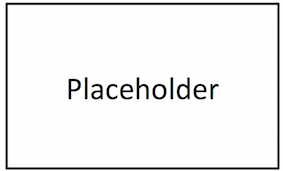
\includegraphics[width=0.9\columnwidth]{figures/placeholder.png}
%\caption{\fix{(Add the figure)} 
%Baseline performance using MKL (and hand) 
%using i-major data layout (not vectorized), for KNL, HSW.}
%\label{fig:tbd}
%\end{figure}

%\begin{figure}%[thbp]
%\centering
%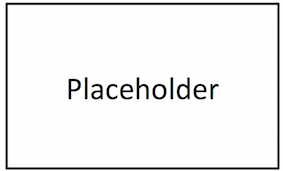
\includegraphics[width=0.9\columnwidth]{figures/placeholder.png}
%\caption{\fix{(Add the figure)} 
%Performance as a function of 32b RCP NR (not needed on KNL), stored
%reciprocal (cuts divides in half) for fixed file size (4?) }
%\end{figure}

%\begin{figure}%[thbp]
%\centering
%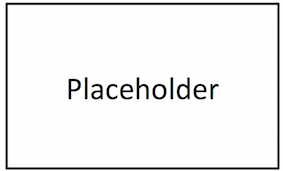
\includegraphics[width=0.9\columnwidth]{figures/placeholder.png}
%\caption{\fix{(Add the figure)} 
%Performance vs. Tile Size (jtile = 1,2,4,8,16,32) }
%\end{figure}

%\begin{figure}%[thbp]
%\centering
%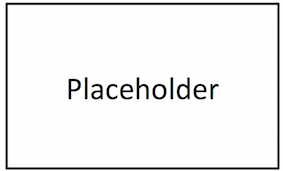
\includegraphics[width=0.9\columnwidth]{figures/placeholder.png}
%\caption{\fix{(Add the figure)} 
%Best Performance vs. MKL using same data layout vs. MKL using its best
%(include DRAM BW limit) }
%\end{figure}

%\begin{figure}%[thbp]
%\centering
%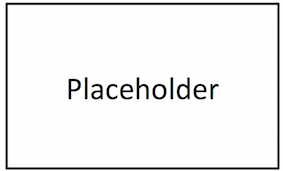
\includegraphics[width=0.9\columnwidth]{figures/placeholder.png}
%\caption{\fix{(Add the figure)} 
%Performance as a function of total parallelism for constant tile size
%[optional time permitting] }
%\end{figure}

%\begin{figure}%[thbp]
%\centering
%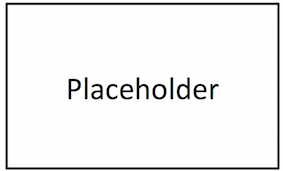
\includegraphics[width=0.9\columnwidth]{figures/placeholder.png}
%\caption{\fix{(Add the figure)} 
%Performance with 2,3,4 hyperthreads...  maybe just prose comments?  }
%\end{figure}

%\begin{figure}%[thbp]
%\centering
%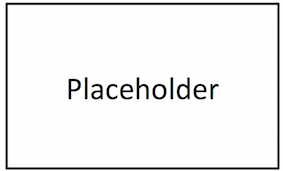
\includegraphics[width=0.9\columnwidth]{figures/placeholder.png}
%\caption{\fix{(Add the figure)} 
%effect of kdim != pow(2)... maybe just prose comments?  }
%\end{figure}

\begin{figure}%[thbp]
\centering
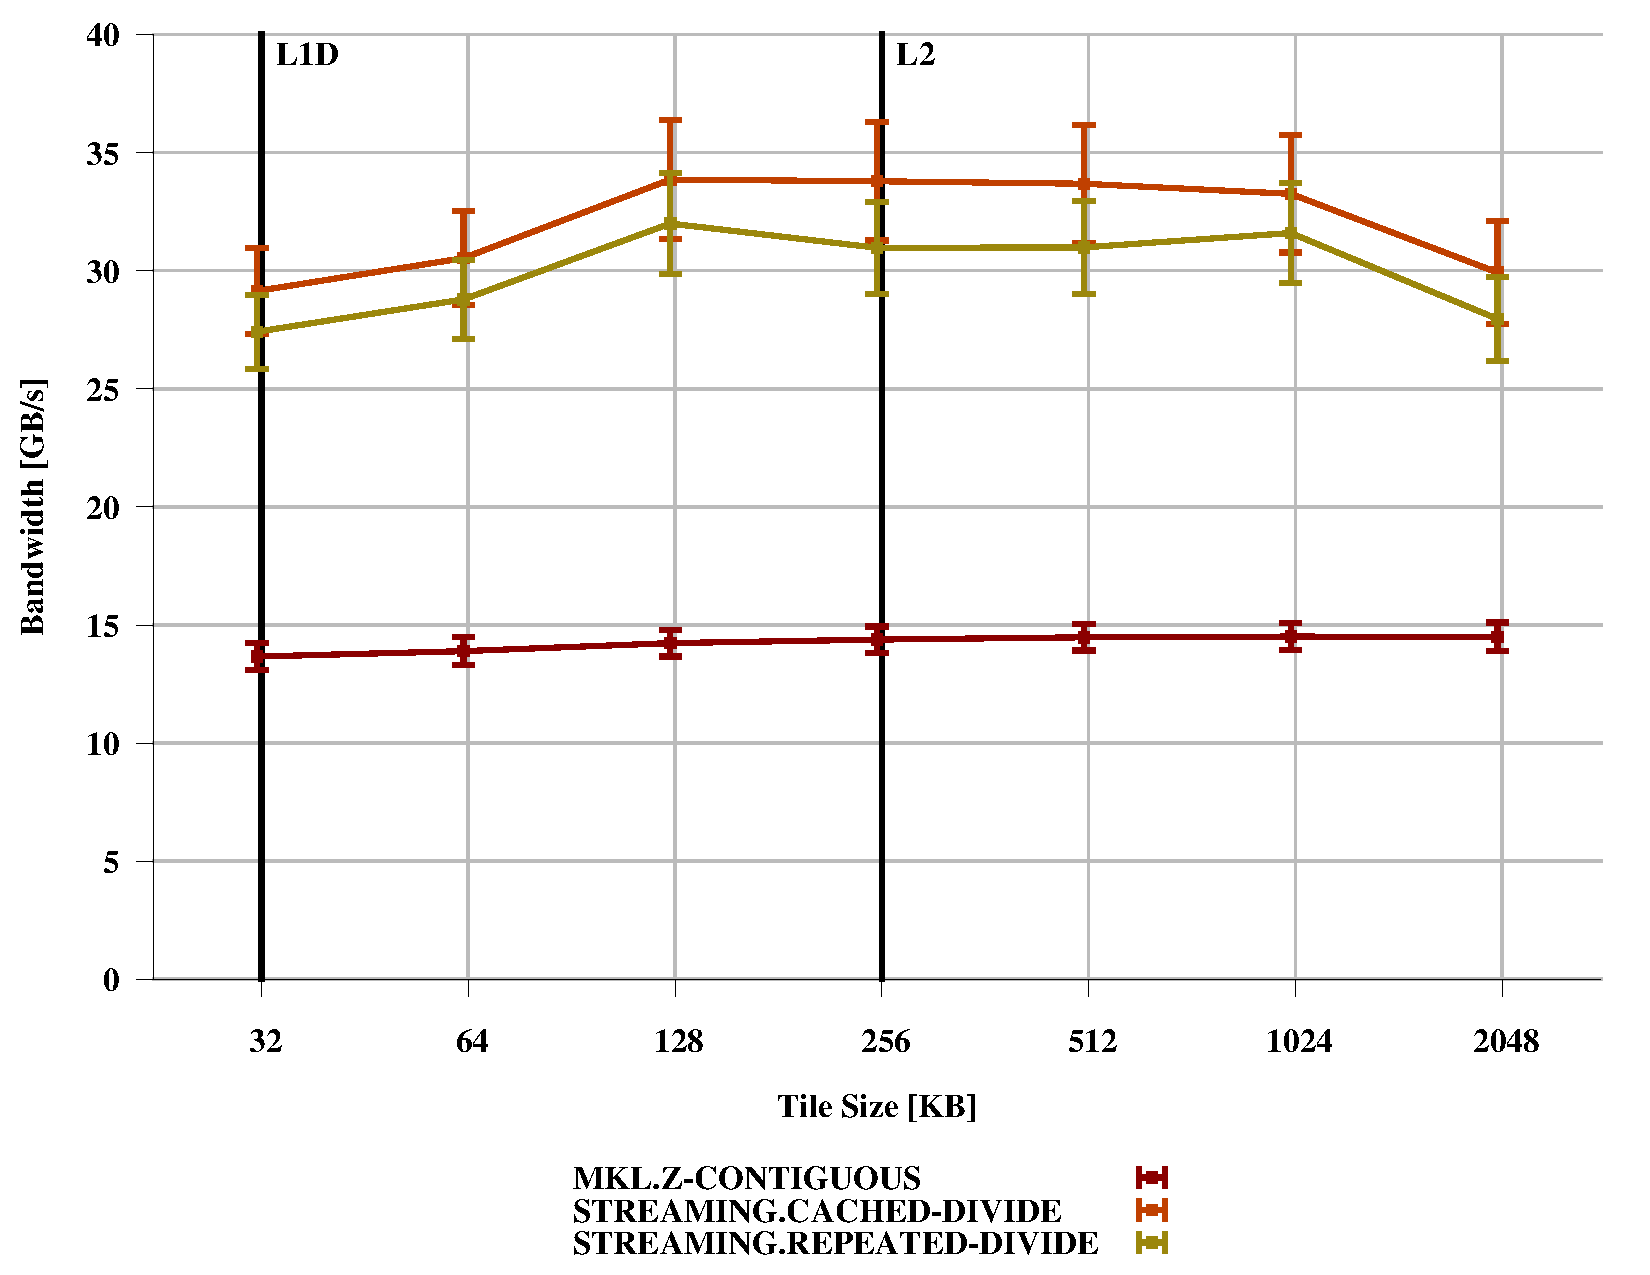
\includegraphics[width=0.9\columnwidth]{figures/post_tsb_tw_sweep_full_matrix_double_precision_production_snb_e5_2670_08_21_2016_8pus.pdf}
\caption{\textbf{Tile Size vs Bandwidth on Sandybridge:}
Measured bandwidth of the tridiagonal solve as a function of tile size on
an Intel Xeon E5-2670 processor. The benchmark was run with 8 threads (each mapped
to a single core of the CPU) and a 7.8 GB problem size. 190 sample runs were
collected.}
\end{figure}

\begin{figure}%[thbp]
\centering
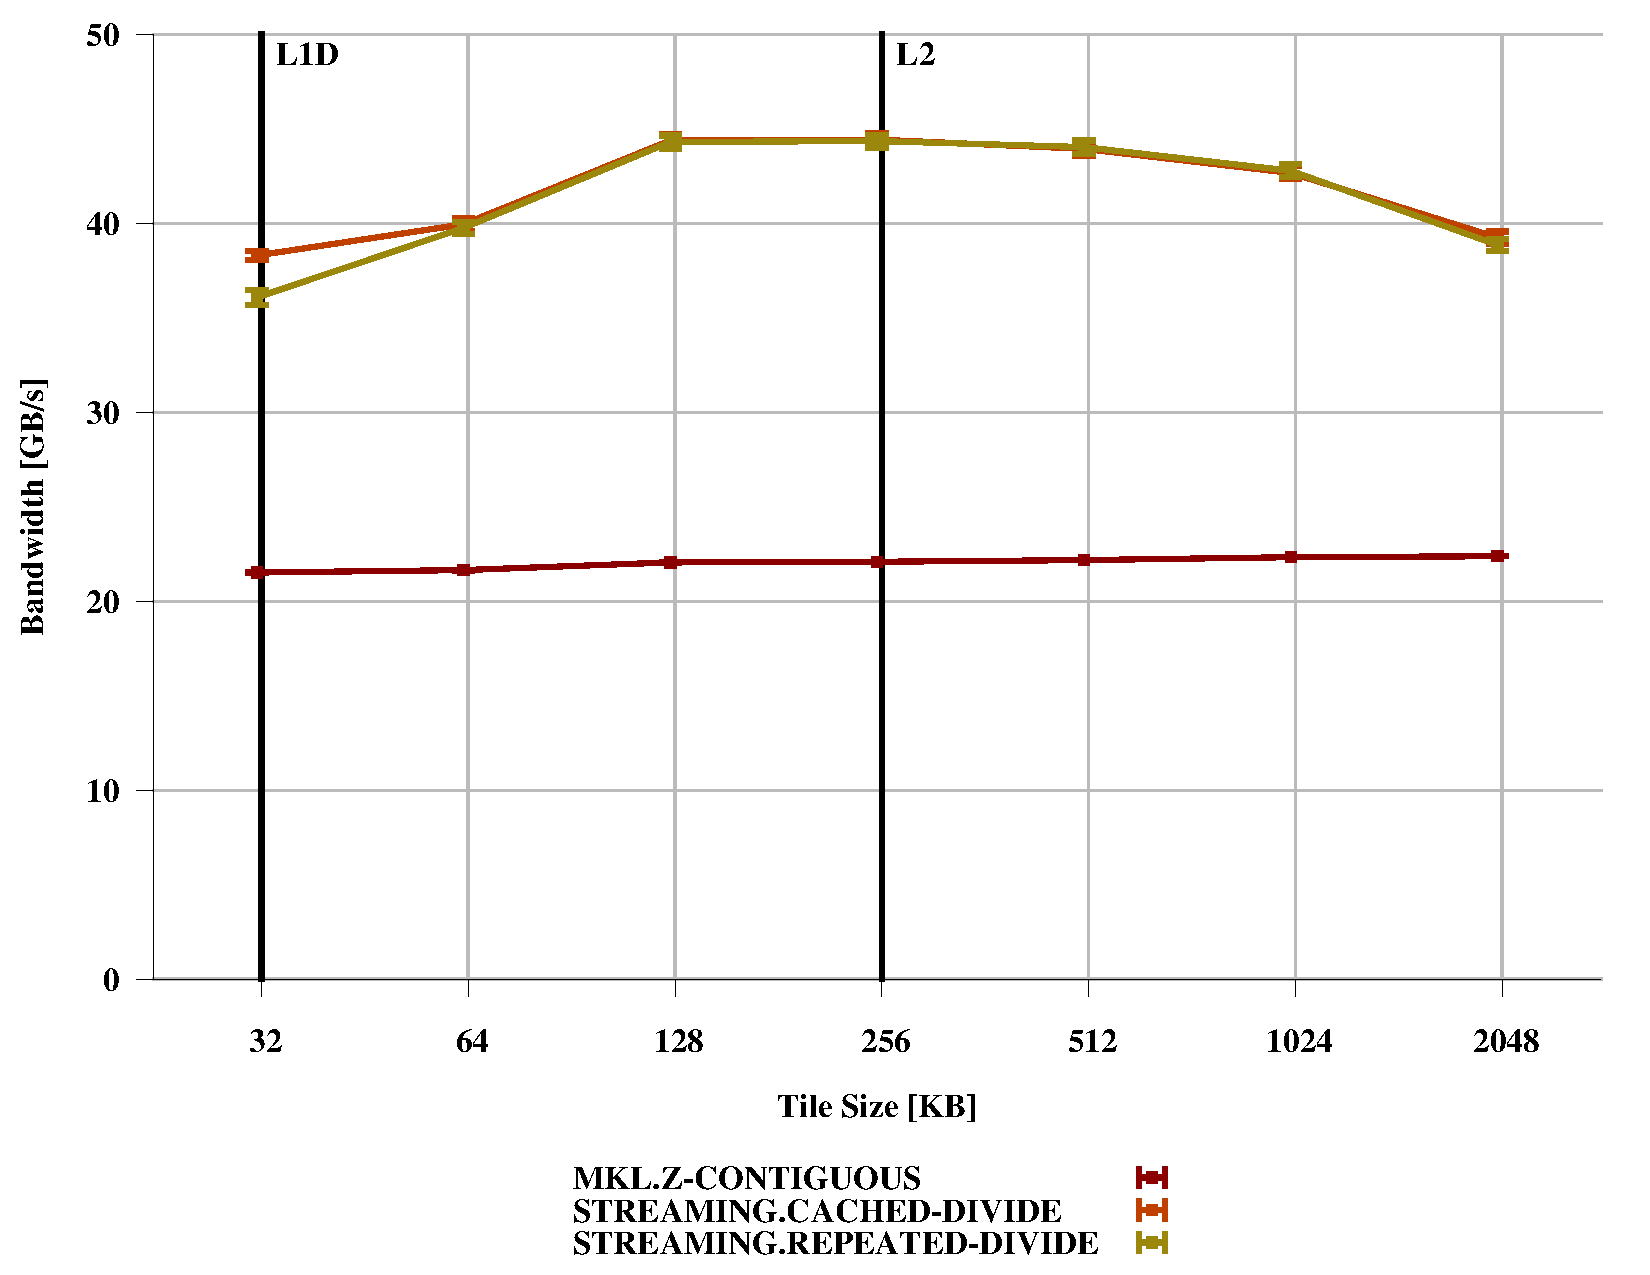
\includegraphics[width=0.9\columnwidth]{figures/post_tsb_tw_sweep_full_matrix_double_precision_production_ivb_e5_2695_v2_08_21_2016_12pus.pdf}
\caption{\textbf{Tile Size vs Bandwidth on Ivybridge:}
Measured bandwidth of the tridiagonal solve as a function of tile size on
an Intel Xeon E5-2695 V2 processor. The benchmark was run with 12 threads (each
mapped to a single core of the CPU) and a 7.8 GB problem size. 160 sample runs
were collected.}
\end{figure}

\begin{figure}%[thbp]
\centering
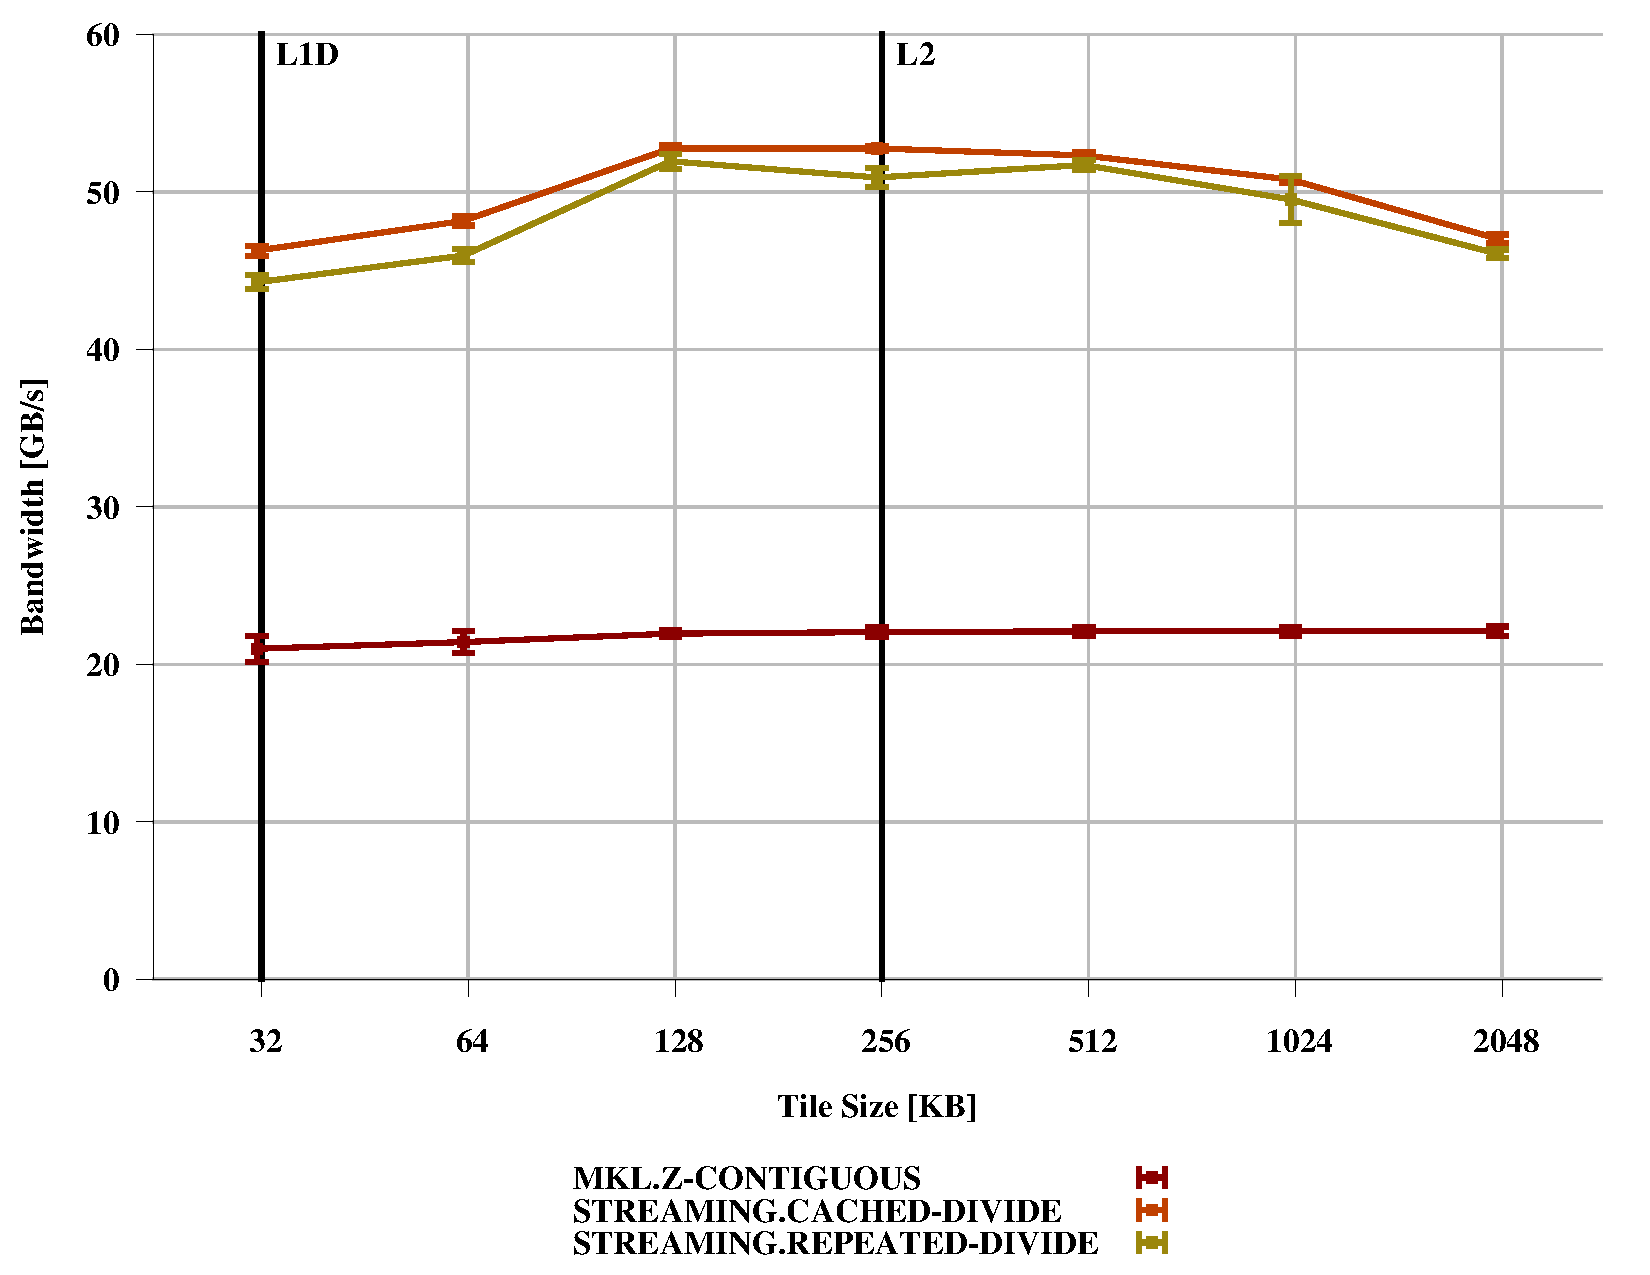
\includegraphics[width=0.9\columnwidth]{figures/post_tsb_tw_sweep_full_matrix_double_precision_production_hsw_e5_2670_v3_08_21_2016_12pus.pdf}
\caption{\textbf{Tile Size vs Bandwidth on Haswell:}
Measured bandwidth of the tridiagonal solve as a function of tile size on
an Intel Xeon E5-2670 V3 processor. The benchmark was run with 12 threads (each
mapped to a single core of the CPU) and a 7.8 GB problem size. 190 sample runs
were collected.}
\end{figure}

\begin{figure}%[thbp]
\centering
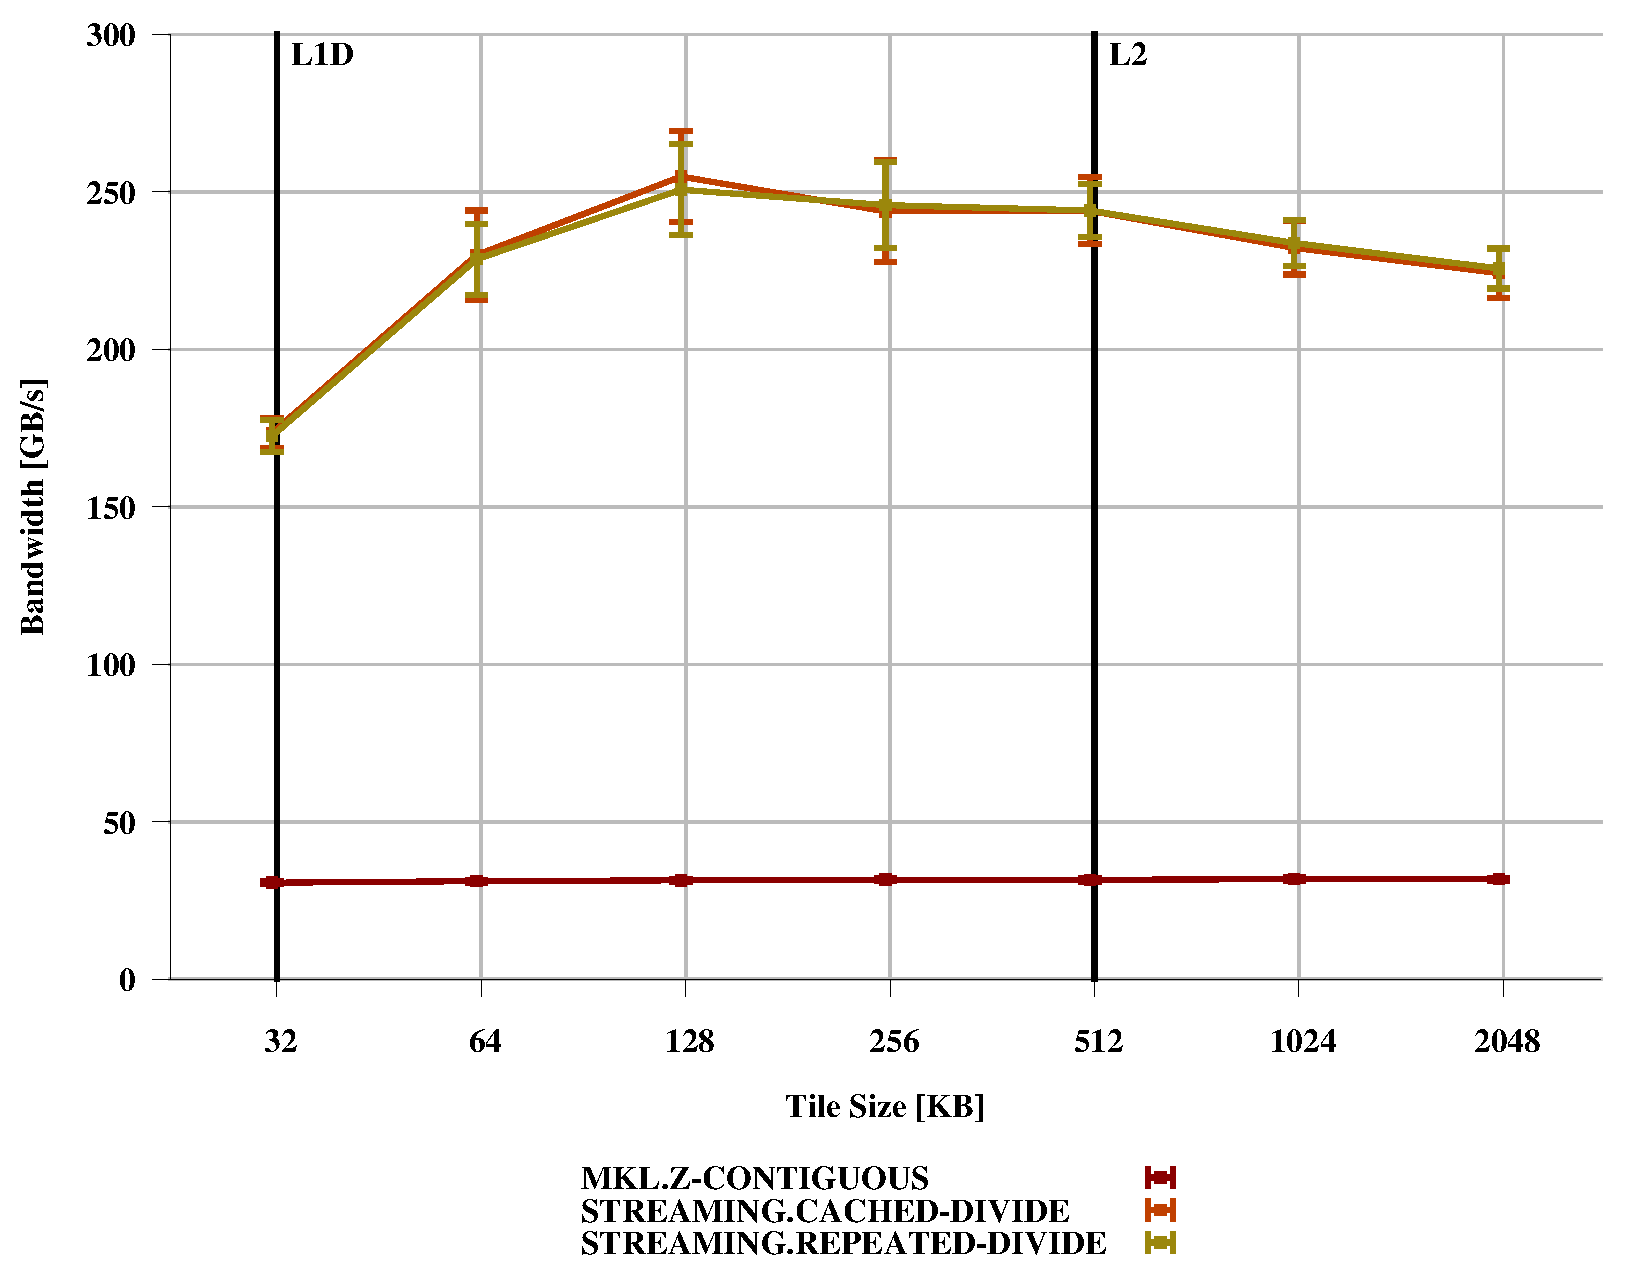
\includegraphics[width=0.9\columnwidth]{figures/post_tsb_tw_sweep_full_matrix_double_precision_production_knl_7210_08_21_2016_64pus.pdf}
\caption{\textbf{Tile Size vs Bandwidth on Knight's Landing:}
Measured bandwidth of the tridiagonal solve as a function of tile size on
an Intel Xeon Phi 7210 processor. The benchmark was run with 64 threads (each
mapped to a single core of the CPU) and a 3.9 GB problem size. 130 sample runs
were collected. The processor was configured in the "quadcache" mode, where the
16GB high-bandwidth memory is configured as a data cache.}
\end{figure}

%===========================================================================
\section{Conclusion}
\fix{Bryce to write}
The conclusion goes here.


%===========================================================================
\section*{Acknowledgments}
\fix{Comment this section out before submitting... Reformat before finalizing...}
\fix{Intel IPCC ack, too}

This research used resources in Lawrence Berkeley National Laboratory and the National Energy Research Scientific Computing Center, which are supported by the U.S. Department of Energy Office of Science's Advanced Scientific Computing Research program under contract number DE-AC02-05CH11231.  
This material is based upon work supported by the U.S. Department of Energy, Office of Science, Advanced Scientific Computing Research, Scientific Discovery through Advanced Computing (SciDAC) program.
%This research used resources of the National Energy Research Scientific Computing Center (NERSC), which is supported by the Office of Science of the U.S. Department of Energy under contract DE-AC02-05CH11231.
%This research used resources of the Argonne Leadership Computing Facility at Argonne National Laboratory, which is supported by the Office of Science of the U.S. Department of Energy under contract DE-AC02-06CH11357.
%This research used resources of the Oak Ridge Leadership Facility at the Oak Ridge National Laboratory, which is supported by the Office of Science of the U.S. Department of Energy under Contract No. DE-AC05-00OR22725.


%===========================================================================
\bibliographystyle{IEEEtran}
\bibliography{sc16-implicit}
%===========================================================================

%===========================================================================
% 

%\section*{Notes/Outline}
%Submission info:
%\url{https://easychair.org/conferences/?conf=pmbs16}
%
%\begin{itemize}
%\item Climate apps use HE-VI model 3D+1D. Also a pattern for 2D+1D and 3D+0D chemistry
%\item Results demonstrate importance of ``batching'' solves, MLK doesn't do
%\item Cache coherency is important: IMEX RK accum, tiling
%\item Explicit part is HO stencil op, memory b/w bound (w/ ghost cells)
%\item Implicit part is non-linear solver: App requires different matrix at each i,j index 
%\item Results in repeated vertical sparse banded solve
%\item Solve (tridiag, banded, dense) should vectorize on i (unit stride), tiled in pencils
%\item Considerations for vector alignment, tiling, and memory
%\item Performance results, scaling, comparison, by platform / parameter
%\item Future work: communication hiding, load imbalance, IMEX
%\end{itemize}
%(Bryce's email comments) Looking over the outline:
%\\
%It's crucial that we clearly identify the optimizations that we
%believe are novel/high-impact, vs the optimizations that are
%well-known to the community (even if they were not well known to us).
%For example, on the outline, we have listed "IMEX RK accum, tiling".
%Do we want to present the accumulation optimizations which removed
%unnecessary temporaries from the time integrator? Do we feel that
%optimization is novel, or is that just a common-sense thing that only
%affected us because of the Chombo programming model? Likewise, do we
%want to present tiling as a focal point in this paper? Tiling is a
%well-known technique; we certainly can't claim tiling in general as
%novel work. Is some part of our tiling approach novel? (how about
%parallelizing the tile loop - is that fairly novel? I know Sam does
%this in HPGMG, but is this a widely used technique?)
%\\
%We would be well served by applying the scientific method at this juncture:
%\\
%\begin{itemize}
%\item Question: What concrete research question(s) are we answering?
%\begin{itemize}
%\item Prior research indicates that HE-VI methods show promise as a
%scalable approach to solving global climate problems on cubed sphere
%geometries because <explanation> [cite prior studies]. How do we
%implement HE-VI methods which perform well on cache-coherent SIMD
%architectures?
%\item When solving a problem with a high horizontal-vertical aspect ratio
%(e.g. the horizontal extents are much greater than the vertical
%extents) with HE-VI methods, it is necessary to perform a large number
%of small vertical implicit solves (<give examples of matrix sizes>
%[citation]) which are independent of each other. <explain the type of
%solves in the climate dycore - e.g. non-linear but nearly banded>
%[citation]. How can we efficiently solve large quantities of small
%non-linear bandedish/banded/tridiagonal matrices on cache-coherent
%SIMD architectures?
%\end{itemize}
%\item Hypothesis: What theories did we come up with that would answer our
%research question(s)?
%\begin{itemize}
%\item Optimal memory access patterns, management of working set sizes
%(e.g. staying in cache) and efficient use of vector units are
%necessary to achieve good performance on cache-coherent SIMD
%architectures.
%\begin{itemize}
%\item Optimal memory access patterns: moving through memory in unit
%stride, controlling the number of streams.
%\item Management of working set sizes: tiling, reducing size of
%temporaries/localizing temporaries (thread-local or otherwise)
%\item Efficient use of vector units: moving through memory in unit
%stride, controlling memory alignment, controlling array strides,
%annotation-assisted autovectorization
%\item TODO: List of individual, concrete optimizations from above.
%\end{itemize}
%\item Mainstream linear algebra libraries (<examples> [citation]) are not
%well-suited for solving large quantities of small non-linear
%bandedish/banded/tridiagonal matrices on cache-coherent SIMD
%architectures because <expalanation> [cite prior studies if possible].
%\end{itemize}
%
%
%\item Prediction: If our hypotheses are true, what results can we expect to
%see? \\
%$\rightarrow$ TODO: What performance characteristics should we see with and
%without each of the concrete optimizations from our hypothesis above?
%
%\item Experiment: Investigate the predictions we've made. \\
%$\rightarrow$ TODO: Methodology for benchmarking the optimizations identified
%above and measuring the performance characteristics we're interested
%in.
%
%\item Analysis: What were the results of our experiments?
%\end{itemize}
%
%List of figures from meeting on 8/11:
%For KNL, HSW, SNB(?)...
%List of figures from meeting on 8/11:
%-For KNL, HSW, SNB(?)...
%\begin{enumerate}
%\item Baseline performance using MKL (and hand) using i-major data layout 
%(not vectorized)
%\item Performance as a function of 32b RCP NR (not needed on KNL), stored
%reciprocal (cuts divides in half) for fixed file size (4?)
%\item Performance vs. Tile Size (jtile = 1,2,4,8,16,32)
%\item Best Performance vs. MKL using same data layout vs. MKL using its best
%(include DRAM BW limit)
%\item Performance as a function of total parallelism for constant tile size
%[optional time permitting]
%\item Performance with 2,3,4 hyperthreads...  maybe just prose comments?
%\item effect of kdim != pow(2)... maybe just prose comments?
%\end{enumerate}


\end{document}


